\documentclass{article}
\usepackage{fancyhdr}
\usepackage{graphicx}
\usepackage{hyperref}
\usepackage{booktabs}
\usepackage{array}
\usepackage{amsmath}
\usepackage[table]{xcolor}
\usepackage{xcolor}
\usepackage{longtable}
\usepackage[a4paper, margin=1in]{geometry}
\usepackage{caption}
\usepackage{ulem}


\pagestyle{fancy}
\fancyhead[L]{User Manual : \textit{Drilling Machine Digital Twin}}
\fancyfoot[L]{Lin Jérôme}
\fancyfoot[C]{
    \begin{minipage}{1.5cm}
        \centering
        
\includegraphics[width=1cm]{SaipemLogo.png}
    \end{minipage}
}
\fancyfoot[R]{\thepage}





\renewcommand{\footrulewidth}{0.1pt}
\renewcommand{\sectionmark}[1]{}
\renewcommand{\subsectionmark}[1]{}
\renewcommand{\contentsname}{}





\title{\textbf{User Manual}\\
\textbf{\textit{Drilling Machine Digital Twin}}}
\author{
    \begin{minipage}[c]{\textwidth}
        \centering
        
\includegraphics[width=4in]{DrillingMachineDigitaTwinLogo.png} \\
        \vspace{2cm}
        
\includegraphics[width=1.5in]{SaipemLogo.png}
    \end{minipage}
}
\date{}




\begin{document}

\maketitle

\vfill
\begin{center}
    \textbf{Lin Jérôme}\\
    \textbf{Saipem SA}
\end{center}






\subsection*{Summary}
\tableofcontents





\newpage
\section{Introduction}\hfill

This user manual provides guidance for interacting with a simplified digital twin of a drilling machine, developed using the Unity game engine as part of an engineering internship project at Saipem SA supervised by Rudy Mauge. The digital twin is designed to simulate the functionality of a real-world drilling machine in a virtual environment, enabling users to explore its components and operations in an interactive and intuitive manner.\\

In addition to interaction, the system allows real-time visualization of sensor data collected from the physical drilling machine. This integration of monitoring and simulation supports a better understanding of machine behavior, facilitates training, and contributes to operational insight in a safe and controlled setting.





\newpage
\section{Installation}\hfill
\begin{itemize}
    \item Download the installer (DM-DigitalTwinSetup.exe)
    \item Run the installer (DM-DigitalTwinSetup.exe) and follow the instructions
    \item Follow the instructions of the installer:
    \begin{itemize}
        \item Choose your preferred language
        \item Accept the terms and conditions
        \item Select the installation directory (default: C:\textbackslash{}Program Files\textbackslash{}DrillingMachine-DigitalTwin)
        \item Choose whether to create a desktop shortcut or not by checking/unchecking the option
        \item Click Install 
    \end{itemize}
    \item After installation:
    \begin{itemize}
        \item Optionally check ”Launch Drilling Machine Digital Twin”
        \item Click Finish to close the installer
    \end{itemize}
\end{itemize}
You can launch the software in two ways:
\begin{itemize}
    \item From the desktop (if shortcut was created):\\Double-click the Drilling Machine Digital Twin icon.
    \item From the Start Menu:\\Go to Start $>$ Drilling Machine Digital Twin $>$ Open
\end{itemize}





\section{Uninstallation}\hfill

\noindent Open Control Panel $>$ Programs $>$ Uninstall a program\\
Select DrillingMachine-DigitalTwin and click Uninstall\\
Or:\\
Use the Uninstall DrillingMachine-DigitalTwin shortcut from the Start Menu





\newpage
\section{Commands}
\subsection{In Drilling Mode}
\begin{table}[h]
    \begin{tabular}{|l|l|l|}
        \hline
        \textbf{Action} & \textbf{Key (QWERTY)} & \textbf{Key (AZERTY)}\\
        \hline
        Return / Settings Menu & ESC & ESC\\
        \hline
        Open Parameter Menu & Tab & Tab\\
        \hline
        Move camera view & Mouse Right Click + Mouse Movement & Mouse Right Click + Mouse Movement\\
        \hline
        Height Navigation & W/S & Z/S\\
        \hline
        Zoom in/out & Mouse scroll & Mouse scroll\\
        \hline
        Select Slip Table & 1 & \&\\
        \hline
        Select Rotary Table	& 2 & é\\
        \hline
        Reset selection & 3 & "\\
        \hline
        Move selected upward & Arrow Key Up & Arrow Key Up\\
        \hline
        Move selected downward & Arrow Key Down & Arrow Key Down\\
        \hline
        Change Drilling Leader Tower details visibility	& V\\
        \hline
        Change Terrain Layer visibility & T\\
        \hline
    \end{tabular}
\end{table}

\subsection{In Replay Mode}
\begin{table}[h]
    \begin{tabular}{|l|l|l|}
        \hline
        \textbf{Action} & \textbf{Key (QWERTY)} & \textbf{Key (AZERTY)}\\
        \hline
        Return / Settings Menu & ESC & ESC\\
        \hline
        Move camera view & Mouse Right Click + Mouse Movement & Mouse Right Click + Mouse Movement\\
        \hline
        Height Navigation & W/S & Z/S\\
        \hline
        Zoom in/out & Mouse scroll & Mouse scroll\\
        \hline
        Change Drilling Leader Tower details visibility	& V & V\\
        \hline
        Change Terrain Layer visibility & T & T\\\
        \hline
    \end{tabular}
\end{table}





\newpage
\section{Mechanics}
\subsection{Main Menu}\hfill

Upon launching the software, users can choose between two modes: Interactive Mode and Replay Mode, by selecting the corresponding button. \\

Additionally, users are directed to the Settings Menu, where various configurable options are available. These include:
\begin{itemize}
    \item Display Settings: Screen mode and refresh rate.
    \item Navigation Sensitivity: Mouse control, scroll sensitivity, and height navigation sensitivity.
    \item Graphics Settings: Fog distance and sensor visibility.
\end{itemize}

Users also have access to the Credits Menu, where information regarding the various assets and development tools utilized in the creation of the software is available.

\subsection{Drilling Mode}\hfill

In Interactive Mode, users directly interact with and control the drilling machine through a set of commands.\\

To move the drilling machine, the user must select one of the two available tables: the Slip Table or the Rotary Table. When one of the tables is selected it is highlighted in white.\\

When a table is locked, it is highlighted in orange upon selection. In this state, the Kelly bar and drill bit move together with the selected table, enabling the drilling operation. When a table is unlocked (highlighted in white), it moves independently along the Kelly bar when the user triggers movement using the associated keys. Note that if both tables are locked simultaneously, neither of them will be able to move.\\

Height navigation is divided into three distinct layers: Surface, Underwater, and Underground. Within the underground layer, users can observe the different terrain strata.\\

A Parameters Menu is accessible by pressing the TAB key, allowing adjustment of several drilling machine and terrain subsea soil. These include:
\begin{itemize}
    \item Time speed, enabling acceleration or deceleration of simulated time.
    \item Drilling velocity.
    \item Rotation velocity.
    \item Subsea soil  parameters such as the required weight for each layer and their respective depths.
\end{itemize}

The Settings Menu can be accessed at any time by pressing the ESC key, which also allows returning to the main menu.\\

Sensors installed on the drilling machine are interactive and can be selected with the mouse when highlighted in blue. Selecting a sensor displays its data evolution through a line chart.
\begin{center}
    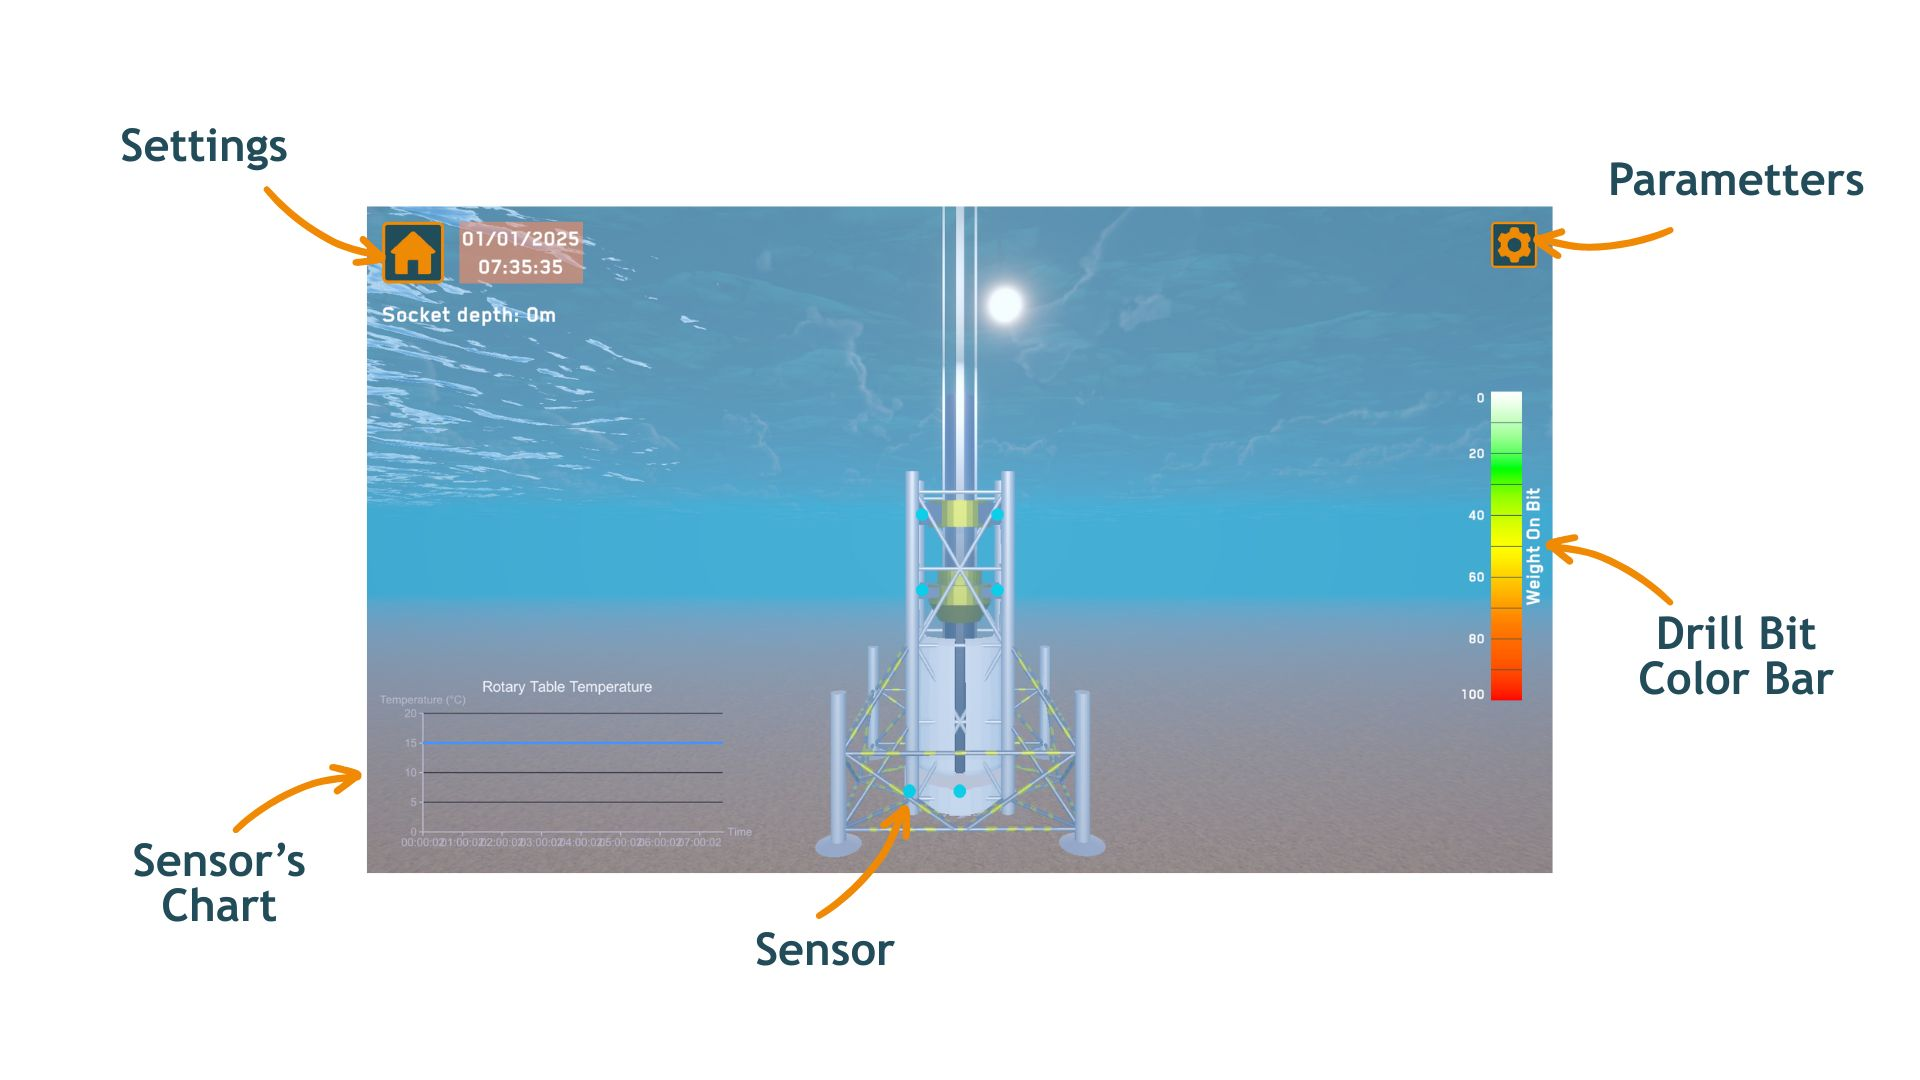
\includegraphics[width=6in]{DrillingMode.jpg}
\end{center}

\subsection{Replay Mode}\hfill

The Replay Mode enables users to review and monitor sensor data and observe the drilling process and installation over time.\\

To use this mode, a properly formatted CSV file containing the required data must be provided. The file must include a header row with the following columns:\\
Date, DLT\_B, DLT\_C, DM, ST\_Height, RT\_Height, DrillBit\_Height, DrillBit\_Rotation, ST\_Load, ST\_Temp, RT\_Load, RT\_Temp, WeightOnBit, DrillingVelocity, DB\_Torque, Layer.\\
\begin{table}[h]
    \begin{tabular}{|l|l|}
        \hline
        \textbf{Variables} & \textbf{Unit/Format}\\
        \hline
        Date & dd/MM/yyyy hh:mm\\
        \hline
        DLT\_B, DLT\_C, DM & Value between 0 and 1\\
        \hline
        DrillBit\_Rotation & RPM\\
        \hline
        ST\_Load, RT\_Load & tons\\
        \hline
        ST\_Temp, RT\_Temp & °C\\
        \hline
        DrillingVelocity & mm/s\\
        \hline
        DB\_Torque & N.m\\
        \hline
        Layer & Integer between 0 and 5\\
        \hline
    \end{tabular}
\end{table}

Sensor data visualization is available through line charts similar to those in Interactive Mode. Users can navigate through the timeline using a slider to move forward or backward to specific timestamps.\\

Replay playback speed can be adjusted, functioning like a video player within a 3D environment.\\

Terrain layers corresponding to the data provided in the CSV file are also displayed.\\

The Settings Menu in Replay Mode offers the same configuration options as in Drilling Mode.
\begin{center}
    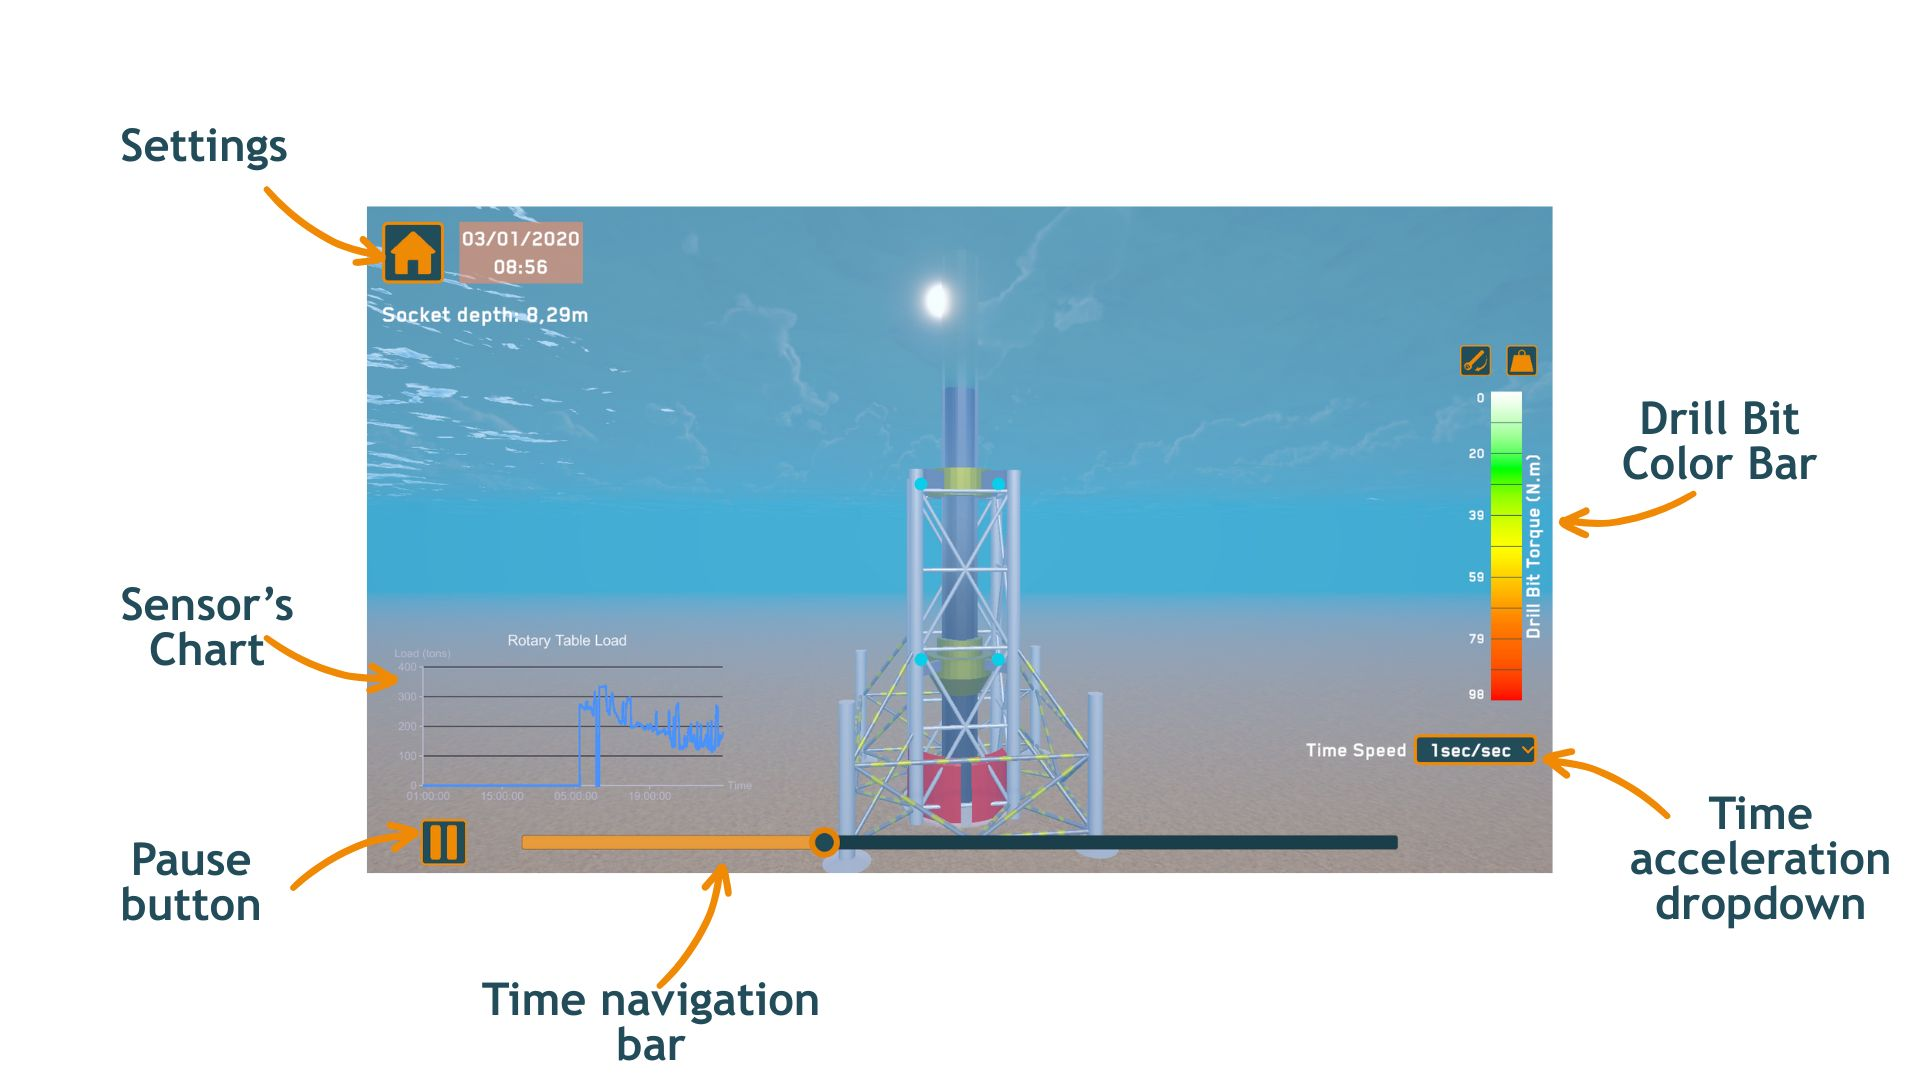
\includegraphics[width=6in]{ReplayMode.jpg}
\end{center}





\section{Step-by-step example}\hfill
\noindent Start the Interactive mode
\begin{itemize}
    \item Launch the Digital Twin
    \item Click on Interactive Mode
\end{itemize}
Change the time acceleration
\begin{itemize}
	\item Go to the parameter menu
	\item Change the Time Speed to “30min/sec”
\end{itemize}
Drill with the slip table
\begin{itemize}
    \item Select the slip table (press 1)
    \item Move the slip table (press Arrow key Down)
\end{itemize}
Drill with the rotary table
\begin{itemize}
    \item Unlock the slip table (press L)
    \item Select the rotary table (press 2)
    \item Lock the rotary table (press L)
    \item Move the rotary table (press Arrow key Down)
\end{itemize}
Move the Drilling Machine Upward
\begin{itemize}
    \item Move the rotary table (press Arrow key Up)
\end{itemize}
See the sensors values
\begin{itemize}
    \item Click on the Rotary Table sensor (click on the blue on one of the blue dots on the rotary table)
\end{itemize}





\section{License}
End-User License Agreement (EULA)\\
\newline
\noindent This software is licensed, not sold. By installing or using the software, you agree to the following terms:\\
1. You may use this software for personal entertainment.\\
2. You may not redistribute, modify, or decompile this software.\\
3. All content, including code, art, and audio, is owned by Lin Jérôme.\\
4. This software is provided "as is", without warranty of any kind.\\
\newline
\noindent © 2025 Saipem SA. All rights reserved.

\end{document}